\evidencelead{E03 · 数据许可 / 人工询问}{我把数据发布边界交给GPT讨论}{争议并非本地实验是否继续，而是教师提供的签到数据能否公开再分发。}
\begin{minipage}[t]{.34\linewidth}
  \centering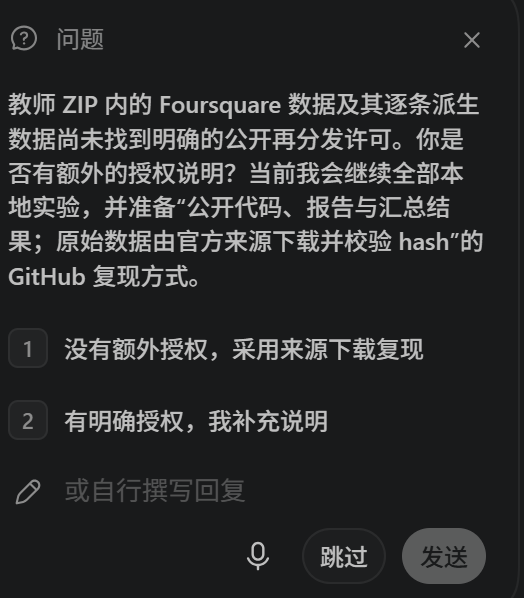
\includegraphics[width=.91\linewidth]{evidence/assets/codex_question_original.png}
\end{minipage}\hfill
\begin{minipage}[t]{.61\linewidth}
  \vspace{3mm}\researchtag{原始Codex权限弹窗}\par\vspace{2mm}
  \small 弹窗提示Foursquare原始记录与逐条派生数据缺少明确再分发授权。我没有让Codex跳过这一问题，而是把真实弹窗交给GPT询问如何处理。\par\vspace{4mm}
  \researchtag{处理边界}\par\vspace{1mm}
  \small 在无法证明公开许可时，保留本地完整实验，公开可复现代码、输入校验和不泄露逐条记录的汇总结果。\par
\end{minipage}
\sourceband{原图：当轮真实上传附件（亦见视频04:46的缩略图），不是重绘的弹窗}
\noindent
\includegraphics[width=93mm]{evidence/assets/D03_user_license.png}\par
\sourceband{RAW VIDEO 04:46.500 · E03 / USER · “这是codex的弹窗，如何回复”}
\evidenceshot{D03_gpt_license}{GPT的回复方向}{GPT建议选“无额外授权，来源下载复现”；后续Codex按公开/本地分流发布。这里不冒称我曾逐字发送GPT所写的回复。}{34}{119}{36}{C1}
\sourceband{RAW VIDEO 04:48.500 · E03 / GPT AFTER}
